% print no page number
\thispagestyle{empty}

\chapter{Front - End Architecture}

To frontend είναι το πιο σημαντικό κομμάτι της εφαρμογής για τον χρήστη. Αν η εφαρμογή ήταν ένα σπίτι, το frontend θα ήταν η εξωτερική πρόσοψη του σπιτού και η οικοδεσπότης, ο οποίος καλωσορίζει τους ανθρώπους μέσα.  Το frontend είναι το κομμάτι της εφαρμογής που χρησιμοποιεί ο χρήστης για να αποκτήσει, να μεταβάλλει και να αποθηκεύσει δεδομένα. Στην συγκεκριμένη εργασία, το frontend είναι αποκλειστικά μια web εφαρμογή.
\newline
Όλη η επίδραση με τον χρήστη γίνετε μέσω του frontend, γιαυτό η σχεδίαση του αποτελεί το δεύτερο βήμα στην υλοποίηση της εφαρμογής. Η τεχνική υλοποίηση του θα γίνει μετά την τεχνική υλοποίηση του backend καθώς η λειτουργικότητα του στηρίζετε στα API calls που προσφέρει το backend.

% leave 60mm empty space below
\vspace{60mm}

\section{Στόχοι της σχεδίασης}
Οι αρχές που ακολουθεί η σχεδίαση του frontend χωρίζετε σε δύο ειδών, τις γενικές αρχές και τις αρχές ασφάλειας.
\begin{description}
\item [Γενικές αρχές] Αναφέρονται σε όλο το frontend και στοχεύουν να κάνουν την εφαρμογή απλή και εύκολη για τον χρήστη.
\newline
Μερικές γενικές αρχές:


\begin{itemize}
  \item Σε κάθε σελίδα του frontend, θα πρέπει να είναι ξεκάθαρες οι διαθέσιμες ενέργειες του χρήστη.
  \item Σε οποιαδήποτε σελίδα βρίσκετε ο χρήστης θα πρέπει να μπορεί να πάει σε οποιαδήποτε άλλη σελίδα της εφαρμογής με μία μόνο κίνηση.
   \item Για κάθε ενέργεια του χρήστη θα πρέπει να υπάρχει μια άμεση απάντηση της εφαρμογής, είτε με αλλαγή περιεχομένου, είτε με ενημερωτικό μύνημα κ.τ.λ.
   \item Σε περίπτωση αποτυχίας κάποιας ενέργειας, θα πρέπει να ενημερώνετε με λεπτομέρεια ο χρήστης ώστε να γνωρίζει πως να συνεχίσει. Αυτό περιλαμβάνει την χρήση μυνημάτων που θα εμφανίζονται στην οθόνη, το focus της σελίδας σε συγκεκριμένα πεδία ή δεδομένα κ.τ.λ.
\end{itemize}


\item [Αρχές ασφάλειας] Οι αρχές ασφάλειας αναφέρονται σε συγκεκριμένα κομμάτια του frontend και είναι κυρίως κομμάτι της ασφάλειας των δεδομένων.

\begin{itemize}
  \item Η εφαρμογή θα χρησιμοποιεί προτόκολλα ασφάλειας για την μεταφορά των δεδομένων του χρήστη.
  \item Ο χρήστης θα παραμένει συνδεμένος για πεπερασμένο χρονικό διάστημα και στη συνέχεια θα πρέπει να ανανεώσει την σύνδεση του.
\end{itemize}

\end{description}

\section{Τεχνικά χαρακτηριστικά}

Οι τεχνολογίες που χρησιμοποιούνται σε κάθε εφαρμογή ποικίλουν ανάλογα με τα άτομα που την υλοποιήσανε, τα χαρακτηριστικά και τις δυνατότητες της εφαρμογής.
\newline
Για τις web εφαρμογές, δύο τεχνολογίες αποτελούν αναπόσπαστα κομμάτια τους:

\begin{description}
\item [Hypertext Markup Language (\textbf{HTML})] Αποτελεί την γλώσσα σήμανσης που δημιουργεί τις σελίδες της εφαρμογής.

\item [Cascading Style Sheets (\textbf{CSS})] Η οποία περιγράφει την μορφοποίηση του κάθε αντικειμένου στη σελίδα. 
\end{description}


Σε συνδυασμό με μία client-based γλώσσα, όπως η Javascript, αποτελούν τα συστατικά στοιχεία κάθε web εφαρμογή σήμερα.

\begin{description}
\item [JavaScript (\textbf{JS})] Είναι μια client-based γλώσσα προγραμματισμού, η οποία δίνει δυνατότητα για δυναμικές ιστοσελίδες και εφαρμογές στο διαδίκτυο.
\end{description}

Για την υλοποίηση της εφαρμογής χρησιμοποιήθηκε το web framework \textbf{AngularJS}, ένα δομικό framework για δυναμικές web εφαρμογές. Χρησιμοποιεί την HTML ως γλώσσα προτύπου και επεκτείνει τη σύνταξη της για να εκφράσει σαφώς και συνοπτικά τα στοιχεία της εφαρμογής. Διάφορες  λειτουργίες της AngularJS μειώνουν ένα μεγάλο μέρος του κώδικα που θα έπρεπε να γραφτεί. Βασίζετε στη Javascript, και την επεκτείνει για να προσθέσει επιπλεόν λειτουργίες προς διευκόλυνση του προγραμματιστή.

\subsection{Εκδόσεις}

Η εφαρμογή έχει υλοποιηθεί και δοκιμαστεί, στο κομμάτι του frontend με τις παρακάτων εκδόσεις:

\begin{description}
\item [HTML] 5
\item [CSS] 3
\item [JavaScript] 5
\item [AngularJS] 1.6.*
\end{description}


% leave 60mm empty space below
\vspace{60mm}

\section{Λειτουργίες Frontent}

Στο frontend της εφαρμογής έχουν πρόσβαση όλοι οι χρήστες της  \textit{Ιδρυματικής Συστοιχίας ΑΠΘ} με τα στοιχεία πιστοποίησης του λογαριασμού τους στο \textit{GRID}. Έχουν πρόσβαση στις παρακάτω λειτουργίες:

\begin{description}
  \item[$\bullet$ Σύνδεση] O χρήστης θα παρέχει το username και password που έχει πάρει κατά την εγγραφή του ως μέλος της \textit{Ιδρυματικής Συστοιχίας ΑΠΘ}.\textit{Προσοχή} , η εφαρμογή δεν παρέχει μέθοδο εγγραφής. Η εφαρμογή θα στείλει τα δεδομένα με ασφαλή πρωτόκολλα στο backend για επιβεβαίωση. Αν τα δεδομένα δεν είναι σωστά θα εμφανίσει το ανάλογο μήνυμα λάθους αλλιώς η εφαρμογή θα μεταβεί στο dashboard του χρήστη.
  \item[$\bullet$ Έλεγχος εργασιών] Ο χρήστης μπορεί να δει τις εργασίες που έχει κάνει submit στον cluster, σε τι κατάσταση βρίσκονται και να τις φιλτράρει βάση κατάστασης, ημερομηνίας υποβολής και ονόματος.
    \item[$\bullet$ Υποβολή εργασίας] Σε αυτή την λειτουργία ο χρήστης μπορεί να επιλέξει να υποβάλει το εκτελέσιμο της εργασίας από τον τοπικό του δίσκο ή να δημιουργήσει η εφαρμογή ένα εκτελέσιμο για αυτόν με βάση παραμέτρους που θα επιλέξει. Επίσης μπορεί να υποβάλει αρχεία εισόδου από τον τοπικό του δίσκο ή να δώσει το path που βρίσκονται μέσα στη συστοιχία.
    \item[$\bullet$ Παραλαβή αποτελεσμάτων] Αν κάποια εργασία έχει εκτελεστεί επιτυχώς, μπορεί να επιλέξει να κατεβάσει τα αποτέλεσμα της στον τοπικό του δίσκο μέσω της εφαρμογής.
\end{description}

\section{Σενάρια χρήσης - Use cases}

\subsection{Είσοδος - Login}

Οι χρήστες της \textit{Ιδρυματικής Συστοιχίας ΑΠΘ} μπορούν να συνδεθούν στην εφαρμογή με τα στοιχεία που χρησιμοποιούν και για τις υπόλοιπες επιστημονικές υπηρεσίες που προσφέρει η συστοιχία. Η πρώτη σελίδα της εφαρμογής είναι η σελίδα του \textbf{Login}. Παρακάτω φαίνεται το σενάριο χρήσης για το \textbf{Login} καθώς και μια εικόνα της σελίδας από την εφαρμογή.

\begin{figure}[t]
\caption{Use case - Login}
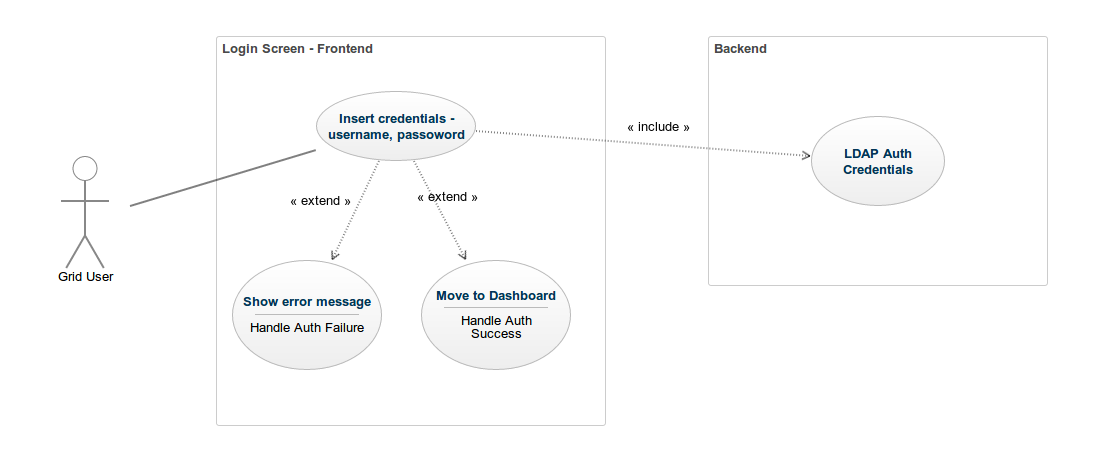
\includegraphics[width=16cm]{../images/login-use-case.png}
\centering
\end{figure}
\clearpage

\begin{figure}[t]
\caption{Screenshot - Login}
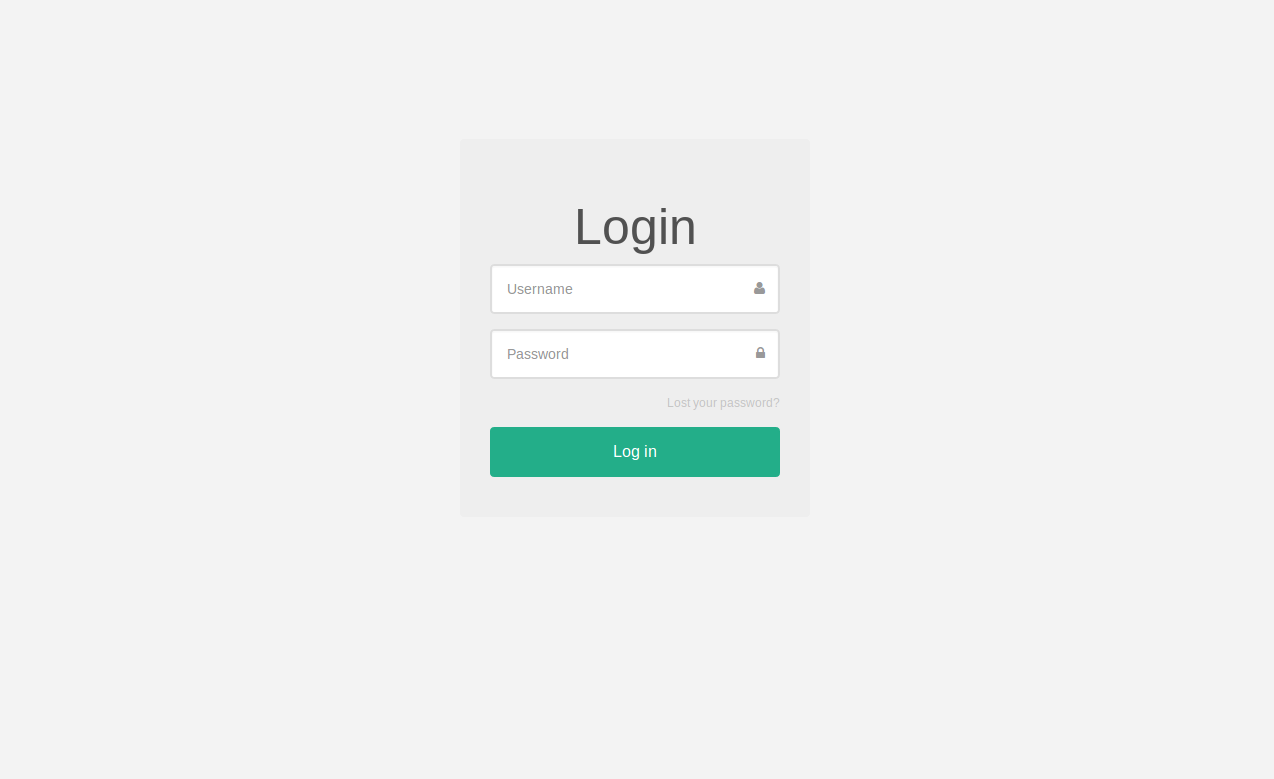
\includegraphics[width=16cm]{../images/login-screenshot.png}
\centering
\end{figure}
\clearpage

Μετά την επιτυχή επιβεβαίωση των στοιχείων, ο χρήστης μεταφέρετε στην κεντρική σελίδα της εφαρμογής.



\begin{figure}[t]
\caption{Screenshot - Home Page}
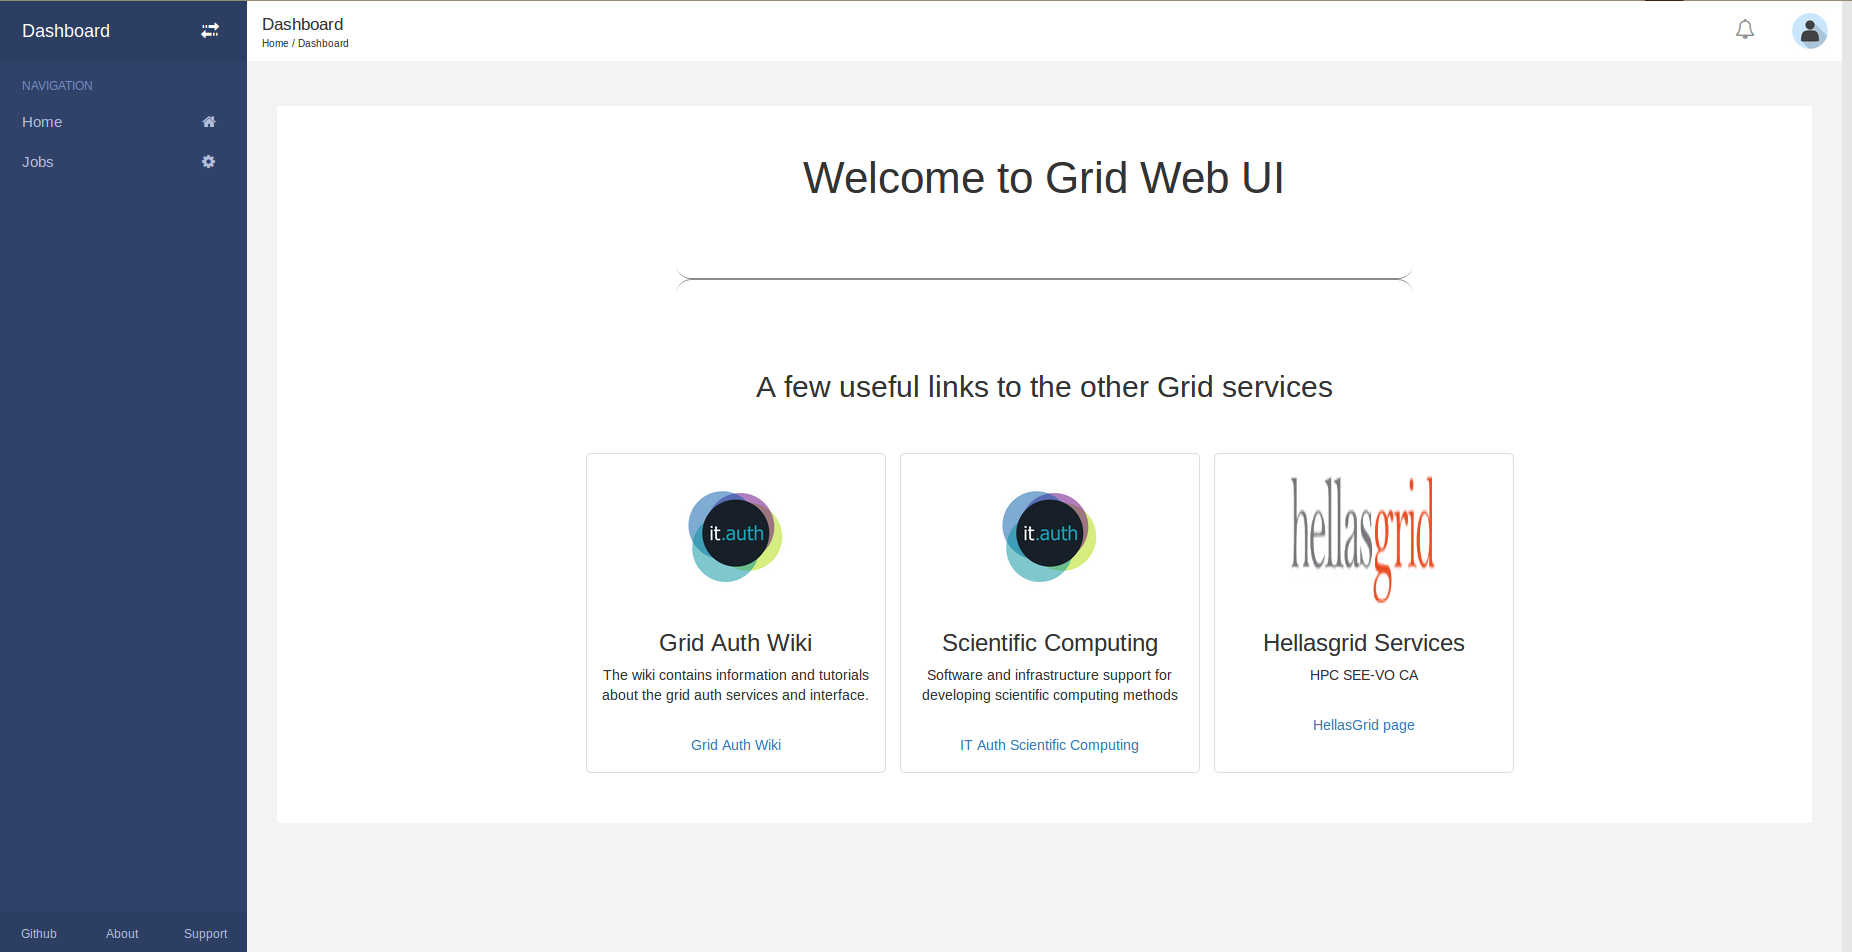
\includegraphics[width=16cm]{../images/home-page-screenshot.png}
\centering
\end{figure}
\clearpage

\subsection{Έλεγχος εργασιών - View jobs}

Από το navigation menu στα δεξιά, της κάθε σελίδας, οι χρήστες μπορούν να μεταφερθούν στην σελίδα προβολής των εργασιών που έχουν υποβάλλει στη συστοιχία.

Αρχικά βλέπουν όλες τις εργασίες που έχουν υποβάλλει, και στη συνέχεια μπορούν να φιλτράρουν τις εργασίες για να δουν όποιες τους ενδιαφέρουν.
\newline
Το φιλτράρισμα μπορεί να γίνει με βάση τρεις διαφορετικούς παράγοντες. 
\newline
Την κατάσταση της εργασίας, η οποία μπορεί να είναι:
\begin{itemize}
\item Running - Η εργασία εκτελείται
\item Finished - Η εργασία έχει ολοκληρωθεί επιτυχώς
\item Stopped - Η εργασία έχει διακόψει την εκτέλεση της πριν ολοκληρωθεί
\end{itemize}
Την ημερομηνία υποβολής της εργασίας, από την πιο πρόσφατη έως την πιο παλιά και αντίστροφα.
\newline
Και τέλος αλφαβητικά με βάση το όνομα της εργασίας.
\newline
Τα φίλτρα μπορούν να χρησιμοποιηθούν και συνδυαστικά για να βγάλουν πιο συγκεκριμένα αποτελέσματα.

\begin{figure}[t]
\caption{Use case - View jobs}
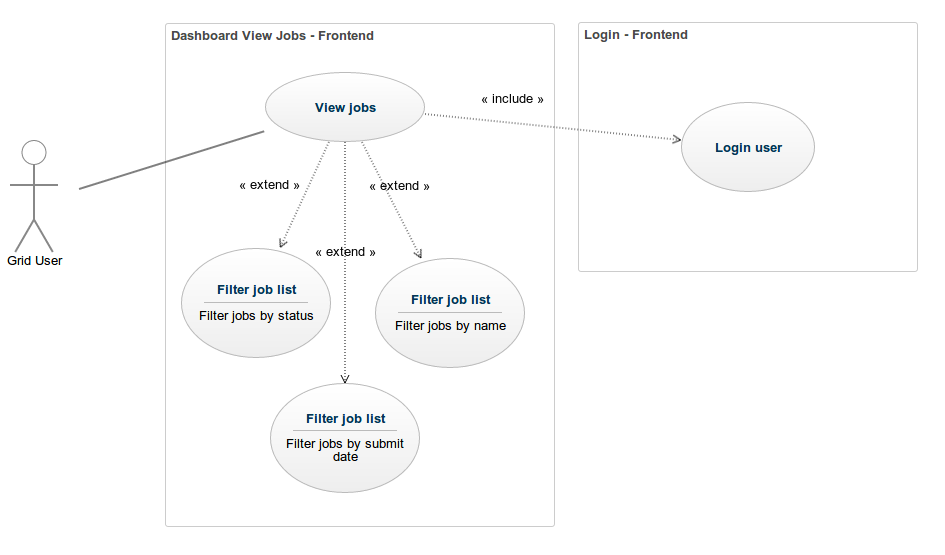
\includegraphics[width=16cm]{../images/view-jobs-case.png}
\centering
\end{figure}
\clearpage

\begin{figure}[t]
\caption{Screenshot - View Jobs}
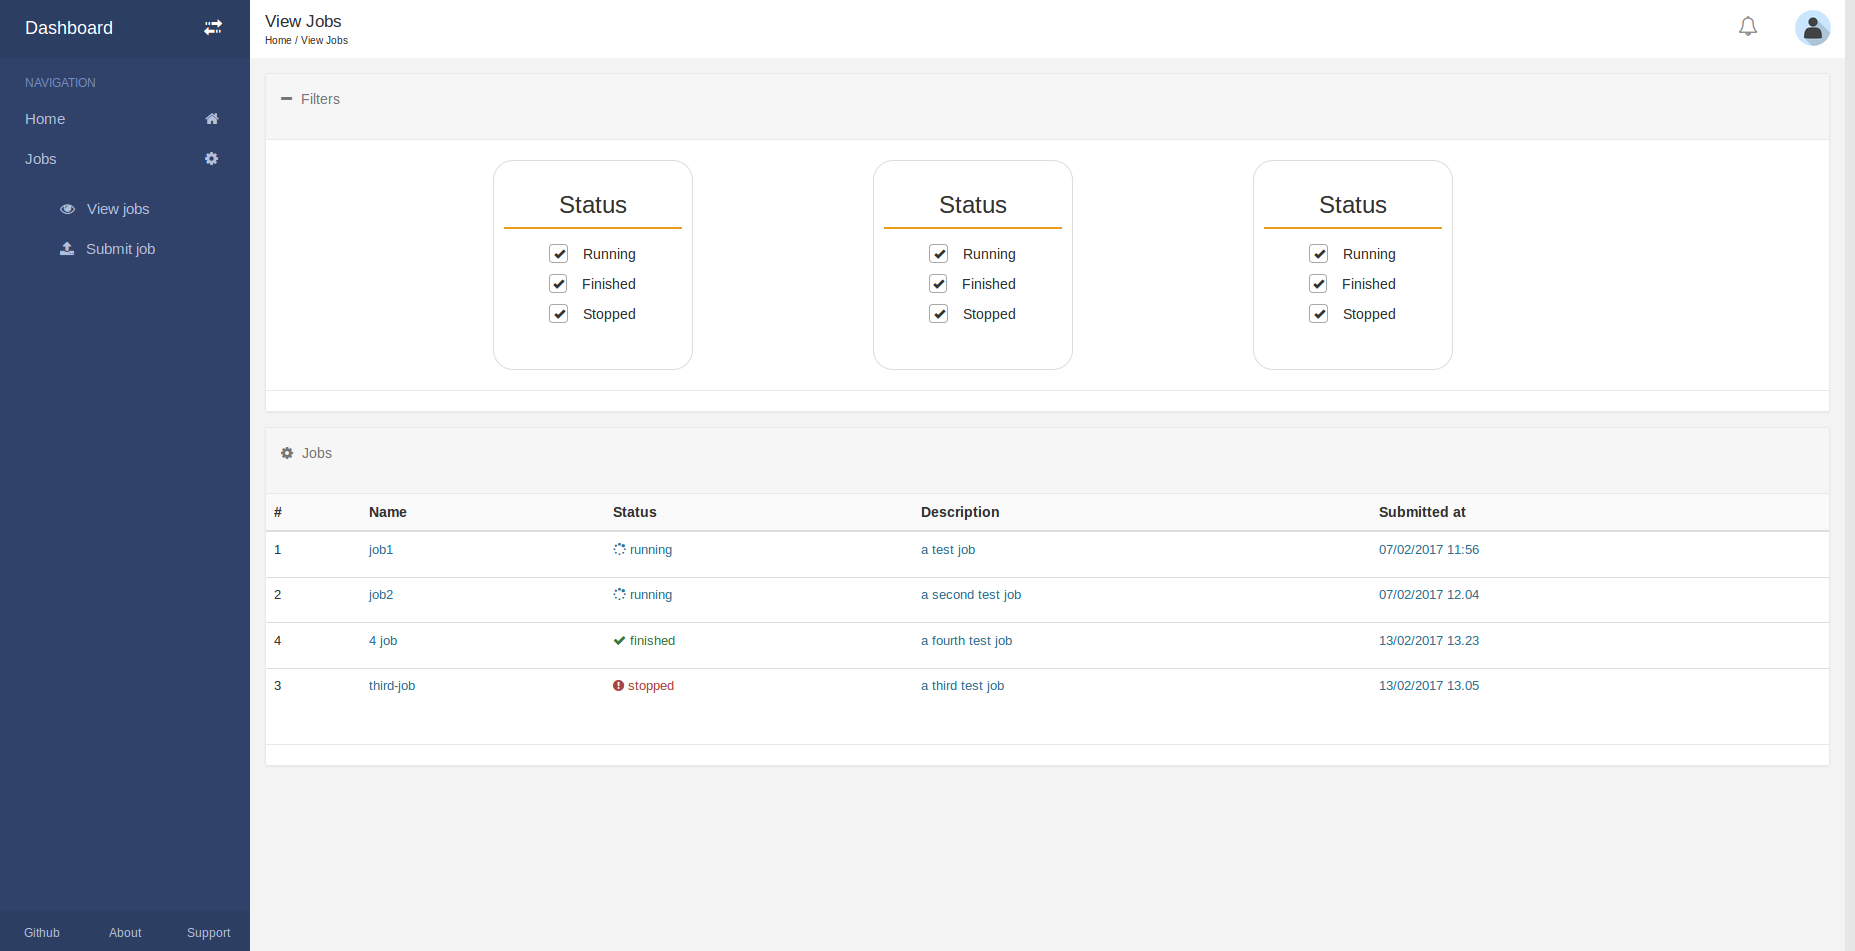
\includegraphics[width=16cm]{../images/view-jobs-screenshot.png}
\centering
\end{figure}
\clearpage







